\chapter{Consideraciones finales}

\section{Título de sección}

Ejemplo de tabla

\begin{table}[h!]
	\centering
	\caption{Leyenda de tabla.}
	\label{tab:comp}
	\begin{tabular}{|c|c|c|}
		\hline
		$t$ (seg) & $x$(t) & $y$(t)\\
		\hline
		1 & 0.0000 & 0.0001\\
		2 & 0.5000 & 0.2498\\
		3 & 1.0000 & 1.0000\\
		4 & 1.5000 & 2.2403\\
		5 & 2.0000 & 4.0010\\
		6 & 2.5000 & 6.2459\\
		\hline
	\end{tabular}
\end{table}

Ejemplo de figura.

\begin{figure}[h!]
	\label{fig:comp}
	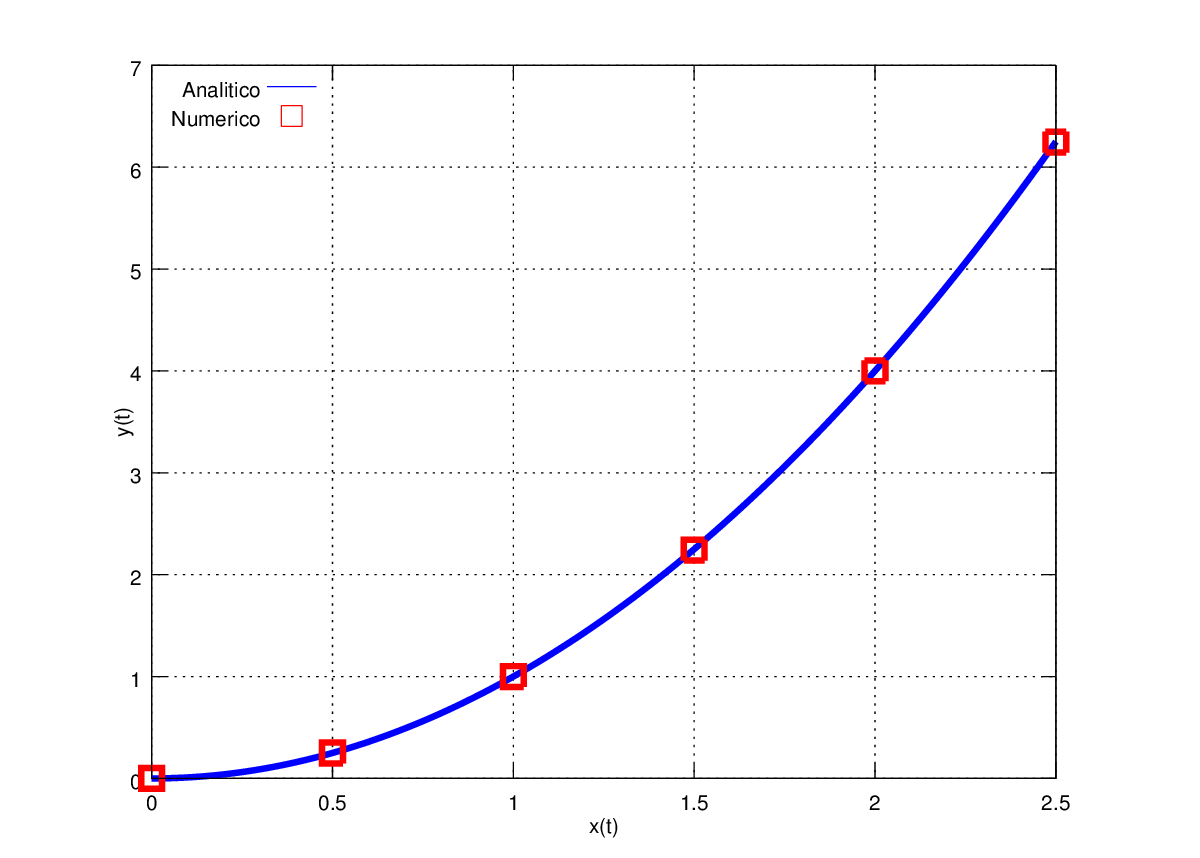
\includegraphics[width=.8\textwidth]{imagenes/chap4/x_vs_y}
	\caption{Leyenda de figura.}
\end{figure}
Ejemplo de ecuación:
\begin{equation}
y(x)=x^2
\end{equation}
En este capítulo se sintetizan las posturas expuestas en el capítulo anterior. Se retoma la pregunta de investigación y se expresa si los resultados apoyan o no la hipótesis planteada. 

Además, se pueden hacer contribuciones teóricas o metodológicas a la disciplina y recomendaciones para trabajos futuros o para profundizar en el campo, plantear nuevas interrogantes o proponer explicaciones \textit{post hoc}. En algunos trabajos este capítulo se subdivide en otras secciones que presentan algunos de los contenidos mencionados. 
En algunas tradiciones académicas este capítulo recibe distintas denominaciones: \textit{Conclusiones}, \textit{Conclusiones y trabajos a futuro}, \textit{Consideraciones finales y recomendaciones}. 

